%\section{Genomics}
%Genomics is a wide area of study focusing on the genomes of organisms
%from all varieties of life. A genome is a sequence of characters that
%contains the fundamental set of `rules' used to create what we know as
%life. One can think of a genome as a set of instructions that our
%cells use in order to complete the tasks that make us function. A
%genome is comprised of tightly bundled sequences of DNA, which are
%stored in the nucleus of cells. These bundles of DNA contain sections
%known as genes, which can be thought of as the tools described by the
%set of instructions. These tools carry out a vast number of processes
%ranging from no known function at all to genes that are key in
%protecting against diseases cancer. Genomes can vary widely in size,
%ranging from small bacterial genomes of roughly 4 Mb up to
%approximately 149000 Mb. Piecing together genomes provides numerous
%opportunities to understand other `omics' within cells, such as
%proteomics, metabolomics, transcriptomics and epigenomics.

Chapter one provides a brief backgound on \textit{Trichoderma} and the context in which is being studied. Section ~\ref{lit:evolution} discusses the evolutionary mechanisms that may have led to the increased production of secondary metabolites in \textit{Trichoderma} species, such as horizontal gene transfer, gene duplication, and transposable elements. 

\section{\textit{Trichoderma} Species and their Evolution}
\label{lit:evolution}

\textit{Trichoderma} are a genus of ascomycete fungi found in a wide
variety of soils, and are well-known for their use in biomanufacturing
of cellulases and hemicellulases as well as their roles as non-toxic,
avirulent opportunistic plant symbionts~\cite{Woo2023}~\cite{Kubicek2019}. 
Many of the features of \textit{Trichoderma}
can be attributed to the large number of secondary metabolites
produced by these fungi, which are used to interact with plants and other organisms in the soil~\cite{Mukherjee2012}. How some \textit{Trichoderma} species evolved to produce more secondary metabolites than others, is a subject of frequent study.

There are many mechanisms organisms may leverage that result in gain or loss of function, and ultimately evolution of a species. One well-studied mechanism is that of horizontal gene transfer (HGT), which is the process of acquiring genetic material from another organism, rather than through inheritance from a parent organism~\cite{Goncalves2024}. HGT is a common mechanism in bacteria, but it has also been observed in fungi, including \textit{Trichoderma} species~\cite{Goncalves2024}. Another mechanism of interest is the duplication of genes, which can result in the production of more than one copy of a gene, leading to increased expression of that gene~\cite{Goncalves2024}. This is particularly relevant in the case of secondary metabolite production, as many \textit{Trichoderma} species have been shown to have multiple copies of genes involved in secondary metabolite production~\cite{Mukherjee2012}. Lastly, transoposable elements (TEs) are another mechanism of interest, as they can insert themselves into the genome and disrupt or enhance the expression of genes~\cite{Goncalves2024}. TEs have been shown to play a role in the evolution of \textit{Trichoderma} species, particularly in the case of secondary metabolite production~\cite{Goncalves2024}. 

Interestingly, both HGT and TEs tend to present themselves in regions where GC content differs from the rest of the genome, ~\cite{Goncalves2024}. Abnormal GC content is also associated with other genomic features, such as centromeres~\cite{Plohl2014} and repetitive regions~\cite{10.1371/journal.pgen.1007467}, both of which may have an effect on the production of secondary metabolites in \textit{Trichoderma} species. As a result, it is important to consider the GC content of a genome when studying \textit{Trichoderma} species, which forms the basis of the Research Question ~\ref{rq:anomalous-sequence-content}.

%One common theory for the increase in secondary metabolites is that \textit%{Trichoderma} initially evolved as a parasite or saprotroph of plants, due to their abundant production of cellulases and plant wall degrading enzymes~\cite{Kubicek2019}. In addition to saprotrophy, \textit{Trichoderma} species are also mycoparasitic, feeding on other Ascomycete and closely related fungal species~\cite{Druzhinina2018}. As a result, it is hypothesized that the elevated production of secondary metabolites in \textit{Trichoderma} arose from the constant change and competition for resources in the environments in which they evolved.~\cite{Mukherjee2012}. While many studies have been conducted on the mechanisms behind fungal evolutionary processes, the process of horizontal gene transfer (HGT), is of particular interest in the case of \textit{Trichoderma}~\cite{Goncalves2024}.
Given the proximity of \textit{Trichoderma} species to other fungi, bacteria, and plants in soils, it is possible that \textit{Trichoderma} species acquired genes which are involved in response to antagonistic and sympathetic intercellular interactions from other organisms. It is also important to note that some \textit{Trichoderma} species have higher numbers of genes involved in secondary metabolite production than others, indicating an evolutionary divergence, making comparative analysis of \textit{Trichoderma} species and strains a useful tool for understanding the mechanisms behind secondary metabolite production~\cite{Mukherjee2012}.

\section{Secondary Metabolites}
\label{lit:secondary-metabolites}

While cellular products essential to an organism's viability are
of great interest, there are a vast number of cellular products that while not
essential, still provide great benefit to the
organism and may be necessary for survival in some situations~\cite{Craney2013}~\cite{Mukherjee2012}. These other cellular products are known
 as secondary metabolites, and they are involved in several roles ranging 
 from cellular signalling to antibiotic activity, making them a frequent 
 subject of study in pharmaceutical research. Enzymes that produce 
 secondary metabolites are comprised of non-ribosomal peptide synthetases 
 (NRPS) and polyketide synthetases (PKS), which synthesize amino acids and 
 other basic enzymatic building blocks~\cite{Komaki2020} into proteins. 
 Genes encoding the NRPSs and PKSs responsible for production of secondary 
 metabolites are often found in clusters within a genome, but their 
 products remain unknown~\cite{Mukherjee2012}. 
 The study of these products is difficult, as the genes encoding the modules that make up NRPSs and PKSs are not expressed under normal laboratory conditions~\cite{Mukherjee2012}. The NRPSs and PKSs that have been studied
 have been shown to be large enzymatic structures containing several 
 functional modules, each responsible for a specific step in the synthesis 
 of a protein~\cite{Mukherjee2012}. 

 Given the modular nature of NRPSs and PKSs, one can assume that many genes are responsible for the production of secondary metabolites. Thus, is is important that methods used for the identification of genes involved in secondary metabolite production are able to identify as many of those genes as possible. Failure to identify these genes may result in an incomplete understanding of the secondary metabolite production process, and may also result in the loss of potential targets for further research. With this in mind, it is important to consider the methods used for identification of genes in a genome, as the methods used can have a significant impact on the results, forming the basis of Research Questions ~\ref{rq:number-of-features} and ~\ref{rq:gene-lengths}. 
 


%\section{Environmental Stress}

%Crop resistance to environmental stressors is a necessity for crop
%health and overall crop yields. Current popular methods for crop
%protection involve the use of pesticides and genetically modified
%organisms, which can be expensive and potentially politically dividing
%in the case of GMOs~\cite{doi:10.1080/10408390600762696}. In addition,
%crops suffer when soils are not sufficient for crop growth and
%health. Soil insufficiencies can result in drought stress as well as
%nutrient stress, leading to poor overall yields.

\section{Novel \textit{Trichoderma} Genomes}

Recently, two strains of \textit{Trichoderma}
have been identified in the prairie regions of Alberta and
Saskatchewan. These two strains, named Tsth20 and DC1, have been found
to have beneficial properties when used as an inoculant for plants in
the soils mentioned before. In addition to these beneficial
properties, the two strains mentioned previously provide even further
protection for plants in dry, salty soils and one strain also has
potential for use as a bioremediation tool in soils contaminated with
hydrocarbon content. Bioremediation and resistance to drought
tolerance has also been investigated in other strains of
\textit{Trichoderma} as well~\cite{10.3389/fpls.2023.1190304}. However,
little is known about the mechanisms at work in these strains, so DC1
and Tsth20 were sequenced by the Global Institute for Food Security
(no publication yet) in an initial attempt to better understand the
details of these genomes. While this research does not eplicitly
identify genomic elements related the beneficial properties of these
genomes, it may serve as a foundation for future research of
\textit{Trichoderma}. The assembly of these genomes come as a result of Research Question ~\ref{rq:assembly-results}.

\section{Gene Predictions and Complementing Similarity Searches}

Gene prediction methods are generally based on the idea that genes can be
identified by searching for patterns in a sequence that match an expected gene structure or model. These gene structures begin from a 5' start codon, continue through a series of exons and introns, and end with a 3' stop codon~\cite{Loftus2003}. While the basic structure of a gene may be present in a sequence, that does not mean that the gene codes for a functional protein, or in the case of secondary metabolites, a protein that produces a secondary metabolite. As a result, gene prediction methods are often used in conjunction with similarity searches, which compare the predicted genes to known genes in other organisms to identify potential functions, and serve as a form of validation for the predicted genes~\cite{Loftus2003}. 

Similarity searches can come in several different forms, such as blast searches, which compare the predicted genes to a database of known proteins, or InterProScan, which compares the predicted genes to a database of known protein domains and binding motifs~\cite{Loftus2003}. These similarity searches can provide additional information about the predicted genes, such as potential functions, and can also help to validate the predicted genes by comparing them to known genes in other organisms. talk about BUSCO tomorrow  

\section{Genome Assembly}

Sequence assembly has been a long-standing problem in the field of
bioinformatics~\cite{Nagarajan2013}. Determining the correct order and
combination of smaller subsequences into an accurate complete sequence
assembly is computationally difficult in terms of compute resources
such as memory, CPU cycles and storage required for input
sequences~\cite{Nagarajan2013}. In addition to these difficulties,
there can be other issues encountered during asssembly due to the
nature of the data or genomes themselves, such as low quality base
calls for long read data, which is not necessarily the case today, or
the inherent content of genomes themselves using repetitive regions as
an example. Insufficient data may result in short, fragmented
assemblies, depending on the size of the genomes, while sequence data
that is not long enough can fail to fully capture repetitive regions
in an assembly. A wide range of assembly tools have been developed
with their own unique approaches to the genome assembly problem, so it
is important to use an appropriate assembler for the task at hand, and
also important to evaluate the assembly thoroughly.

Genome assembly tools generally approach the assembly problem using a
graph-based approach. The most common graph-based approach is the de
Bruijn graph assembly~\cite{Compeau2011}. A graph in this context, is
set of nodes (\textit{k}-mers from sequences) connected by edges
(overlaps between \textit{k}-mers). Traversing through this graph
results in longer subsequences that ultimately result in a set of
sequences referred to as an assembly. In the early years of long read
sequence data, sequencing platforms encountered difficulties producing
consistently high scores for base calls when sequencing. To combat
this, some assembly workflows may also include a polishing or
correction step once the initial assembly is completed in which high
quality short read sequences are used as supplemental information to
correct low quality regions in the assembly. These low quality base
calls are typically not present in modern long read sequencing
approaches as the methodology and quality of calls have improved
drastically. While the polishing step is arguably unnecessary in
modern assemblies, the polishing programs remain available should
researchers be interested in applying additional reads for polishing.

One approach to aid in the previously mentioned issue of assembly
correctness is to use a combination of long and short reads in what is
known as a hybrid assembly. Combining both highly accurate short reads
with deep coverage along with less accurate but much longer reads can
produce high quality genome assemblies that capture long repetitive
regions. Hybrid assembly approaches have been shown to produce high
quality assemblies in a wide variety of organisms as the combine long
read data with short data to produce assemblies that properly
represent long repetetive regions with additionaly high quality
Illumina sequences for correction. Once assembled, the sequences must
also be evaluated with measures such as N50, L50, coverage, average
contig length and total assembled length to ensure that the genomes
are well assembled, at least based on these
metrics~\cite{Nagarajan2013}. Following appropriate assembly protocols
is essential to the further success of a project as downstream
processing such as annotation depends on a high-quality assembly.

\section{Identification of Anomolous Genomic regions}
One important aspect of interest when assembling any form of sequence
is GC content or percent GC of the assembled sequence. Large regions
of anomolous GC content may be of interest to researchers as they may
contain repetitive regions and unique features responsible for traits
specific to the organism in question.



\section{Gene Finding Methods}
Gene finding (or gene annotation) has been a long standing
computational problem in bioinformatics, which concerns itself with
identifying potential genes within assemblies based on patterns or
pre-existing experimental evidence considered by the gene finding
program. This process is critical for unraveling and understanding the
complex processes occurring in all forms of life. In a general sense,
gene finding programs operate by searching for patters or indicators
showing that a gene of feature may be present. The most basic
indicators being start and stop codons, with splice sites in
between should the sequence match the applied model. The results
produced by gene finding tools can vary considerably for a number of
reasons, including quality of the assembly, the intrinsic model used
by the gene finder, filtering criteria, and even the nature of the
organism and assembly itself. Given the broad applications, choice of
gene finding tools, and the variability of assemblies being
considered, it is important that we gain a deeper understanding of
these tools prior to putting them to use.

There are two common methods for gene finding, those methods being
\textit{ab initio} methods, where programs search for patterns and
gene structures, and similarity or evidence-based searches, which use
prior information such as RNAseq data, expressed sequence tags and
expressd protein sequences to identify genes within a new
genome~\cite{Ejigu2020}. Complicating the process more is the
introduction of introns and alternative splicing in eukaryotes, making
it possible for one gene to have several possible transcripts at the
same locus. An example of an \textit{ab initio} method would be
GeneMark-ES~\cite{10.1093/nar/gki937}, while an evidence based tool
would be Braker2~\cite{Bruna2021}.
\textit{Ab initio} gene finders typically predict genes using a Hidden
Markov Model (HMM)~\cite{Ejigu2020}. These predictions are based on
`signals' or features associated with a gene, such as the usual start,
stop, exon and intron portions of a gene as well as upstream promoter
sequences and more. In this case, these signals would be considered
states in the terminology associated with HMMs. Gene finders wish to
predict these states based on observations, or sequences presented to
the model. HMMs in gene finding tools are trained beforehand and then
applied to a sequence. This means that a gene finding program may not
be trained in the context of any assembly provided to it, and thus may
miss genes that are unique to the assembly in question.
On the other hand, while still relying on HMMs for a `base' set of
predictions, evidence-based gene finding tools leverage new evidence
that may be outside the scope of the pre-existing
model~\cite{Keller2011}.  As an example, an evidence-based model would
be useful in a situation where you are interested in annotating a new
assembly for a non-model organism. The addition of experimental data
provides context specific to your assembly of interest while still
retaining the predictions from existing HMM models.

There are also other aspects of gene finding tools that are important
to consider. These include features such as whether or not the gene
finders find non-coding RNAs, annotation of 5' and 3' UTR regions, and
in the case of ab-initio methods, the assumptions made by the
underlying models used for gene finding. These features and others can
influence a user's decision on which gene finding tool to consider and
will complicate comparative analysis of multiple gene finding
tools. (citation needed somewhere in here)

%\section{Repeat Identification and Masking}
%Repeat identification within assembled genomes is a problem that needs
%to be considered during the genome annotation process. Regions with
%long repeats can have a significant impact on genome assembly as well
%as gene finding due to the limitation of short reads used in some
%assemblies~\cite{Treangen2011}. Short reads may be unable to bridge or
%cover entire repeat regions within a genome, so it is important to
%consider the use of long reads from technologies such as Nanopore or
%PacBio\texttrademark ~\cite{Rhoads2015} to provide a complete picture of
%these regions when pursuing a new genome assembly project. It is also
%possible for repetitive regions to contain genes as well, making for
%an interesting investigation in regards to \textit{Trichoderma}, as
%fungal genomes have been shown to contain many repeat regions with a
%high concentration of A and T
%nucleotides~\cite{10.1371/journal.pgen.1007467}. Once these repetitive
%regions have been identified, the genome could be masked as a method
%to mark these regions for downstream processing if desired, as these
%regions may be poorly assembled and may result in found genes that do
%not truly exist in those regions. However, this may not be as common
%today, as repetetive regions have been shown to contain genes as
%well~\cite{Slotkin2018}. This may affect the gene finding process
%described later and may be an interesting topic to look into
%considering the large number of available gene finding programs.

%\section{Centromere Identification}
%A centromere is a region of a chromosome that is crucial for the
%proper cell division. These regions are the main anchor for
%microtubules, which are fibers that attach to centromeres to separate
%chromosomes during both mitosis and meiosis. Centromeres are critical
%to the survival of an organism, with malfunctions in the process of
%cell division usually resulting in potential disease and fatal
%outcomes~\cite{Plohl2014}. Centromeric sequences can be comprised of
%several different genetic components, with repetititve regions being
%the most prevalent in the forms of satellite DNA and transposable
%elements. In addition to centromeric regions, there are flanking
%pericentric regions with their own properties, including potential
%candidates for small-interfering RNAs~\cite{Plohl2014}. Identification
%and consideration of centromeric regions may prove useful when
%comparing the outputs of gene finding tools, as the underlying
%properties and structure of the genetic sequence differ in comparison
%to typical coding regions of DNA.

%\section{Sequencing}
%Sequencing data is a pivotal form of data used in nearly all
%applications of Bioinformatics. To understand the processes used by
%organisms for survival, we must have an initial set of data points to
%work with. These sequences, referred to as reads after sequencing, are
%the foundation for solving problems ranging from taxonomical
%classification to the understanding or complex biological functions
%like signaling pathways. Reads may come in a variety of forms and
%formats depending on the desired application.

%\section{Whole Genome Shotgun Sequencing}
%Whole Genome Shotgun sequencing (WGS), is a method to produce a large
%number of genomic sequences from a sample of interest for the purpose
%of genome asembly. This is form of sequencing is quite common as it is
%has a wide variety of applications in research~~\cite{Adams2008}. WGS
%involves slicing up genomic DNA into smaller segments. These small
%segments are then processed further resulting in a set of physical
%molecules that can be supplied to a compatible sequencing platform of
%which there are a variety. Modern sequencing platforms are comprised
%of next generation sequencing (NGS) and 3rd generation sequencing
%approaches.

%\section{Next Generation Sequencing - Illumina}
%Illumina\texttrademark ~~\cite{Bennett2004} sequencing is one of the
%most popular NGS platforms currently available. Illumina sequencing
%produces a very large number of high quality short reads, typically
%between 75 and 250 base pairs in length. Sequencing libraries can be
%prepared to produce reads solely from one end of a sequence fragment
%(single-end) or both ends (paired-end). Advantages of paired end
%sequences are the additional context provided by the paired sequence
%on the opposite end of the fragment. This context is leveraged by read
%processing tools to identify features such as repetitive regions and
%genomic rearrangments, which can be significant in downstream
%analyses. Illumina sequence librairies are generated by first
%fragmenting the DNA samples, amplifying them via PCR, ligating
%adapters that allow the sequence to bind to the sequencing plate, and
%finally identifying each fragment's sequence of nucleotides using
%fluorescently-labeled nucleotides that bind to the
%fragments~~\cite{Goodwin2016}.

%\section{3rd Generation Sequencing - Nanopore}

%Nanopore\texttrademark ~~\cite{Wang2021} sequencing data is relatively
%recent approach to sequencing projects. While Illumina reads are
%short, Nanopore reads are much larger, ranging from 10Kb to 300Kb
%depending on the approach used. Long reads are beneficial due to their
%ability to bridge the gaps between difficult to assemble regions when
%performing sequence assembly. An example of a difficult to assemble
%region would be a region with a high repeat content, where a large
%number of small repeats may be collapsed during the assembly process,
%resulting in an assembly that does not represent the true nature of
%the sequence being studied~~\cite{Marx2023}. While Nanopore was
%previously known for having lower quality base calls when compared to
%Illumina, that is no longer the case at this time. Nanopore sequencing
%works by passing long segments of genetic sequence through a membrane
%bound protein and measuring changes in electrical current, which is
%characteristic of the nucleotide at a given position.

%\section{RefSeq}

%First, we will briefly discuss the RefSeq annotation process. RefSeq
%annotation is only applied to data that is submitted to NCBI. The
%RefSeq Eukaryotic Genome Annotation Pipeline~\cite{NCBI2024} is a
%genome annotation process developed and maintained by NCBI. The
%pipeline is not directly publicly available to public users, and
%requires submission of data to NCBI. Once data is submitted to NCBI,
%the RefSeq annotation pipeline may be applied upon request only if the
%genome is the highest quality assembly for the species in question or
%if the genome is of significant interest to the scientific community,
%limiting reach of the annotation process to many users. The pipeline
%supplies existing RNAseq, CDS and protein sequences to NCBI's in-house
%gene prediction tool Gnomon, which produces trained models for gene
%prediction. While the tools used for alignment and processing of
%supporting sequence information are listed, the inner workings of
%Gnomon are not well documented, at least from the public perspective,
%and I was unable to find Gnomon in any compilable or executable form
%during my search. Recreation of the RefSeq pipeline would prove
%extremely challenging if not impossible without supporting
%information. Run times for this pipeline are difficult to determine
%due to the hidden nature of the pipeline, unknown compute resources
%and varying quantities of data used. The RefSeq annotation process
%produces comprehensive outputs, including CDS sequences, translated
%CDS, RNA from genomic sequences, proteins, feature counts and tables,
%and finally GFF and GTF formatted annotation files for these features.

%\section{InterProScan}
%The outputs from gene finding tools are a set of potential genes that
%fit the model used by each tool. While they are considered genes, the
%use of the word gene is used in a very loose sense, in that these
%genes may or may not be functional or match any existing gene
%sequences from previous research. Typically, to confirm the
%'correctness' of predicted genes, the outputs from a given tool are
%used in a sequence similarity search against a reference set of genes
%or a large datasbase comprised of multiple organisms. This approach is
%straightforward, but can introduce bias from database choice and also
%allows for vague or loose matches, depending on the parameters used
%and the interpretation of the results. Another approach is to use
%InterProScan, which is a tool used for functional annotation of
%proteins using evidence from a variety of databases
%~\cite{10.1093/nar/gkac993}. The presence of some form of functional
%domain or annotated structure in a predicted gene sequence is
%reasonable evidence for the existence of a predicted gene. This
%approach also avoids the problems associated with similarity-based
%approaches.


%\section{File Formats}

%\subsection{FASTA}
%One of the most popular formats for sequences of DNA, RNA and amino
%acids is the FASTA format. The FASTA format consists of one or more
%entries containing two or more lines. The first line of an entry is
%the ID line, which must begin with a greater-than (\textgreater)
%character, followed by an ID and any other pertinent inormation for
%the following sequence. The greater-than character is the indicator
%that a new sequence has begun. The following line(s) contain the
%actual sequenced nucleotides or amino acids, which can be contained on
%one line or split across many lines. An example of multiple FASTA
%entries are shown in figure~~\ref{fig:fasta-example}.

%\begin{figure}
%  \centering
%  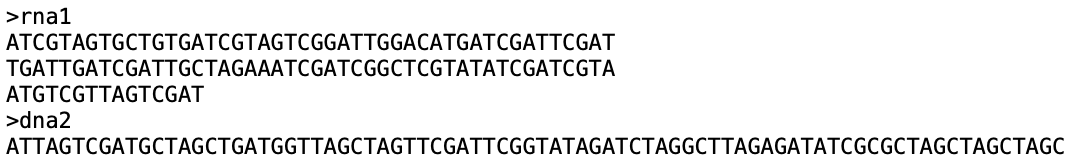
\includegraphics[width=0.8\textwidth]{figures/fasta-example.png}
%  \caption{Example of two FASTA sequence entries. One example with
%    sequence characters split across multiple lines, and one showing
%    all sequence characters on the same line.}
%  \label{fig:fasta-example}
%\end{figure}

%\subsection{FASTQ}
%Another popular sequencing format is the FASTQ format. This format is
%very similar to the FASTA format but with the addition of two more
%lines per sequence entry and a change to the character indicating the
%beginning of a new sequence entry. An example of a FASTQ entry is
%shown in figure~~\ref{fig:fastq-example}. In FASTQ formatted entries,
%the greater-than (\textgreater) character is swapped with the at (@)
%character. The IDs for the sequence also follow a specific format,
%which provide information about the sequencing run and flowcell that
%the read was sequenced on. This information can then be traced back to
%the sequencing experiment in the case that there were errors or
%anomalies in the output from the experiment. Following the ID is the
%string of base calls. The third line in a FASTQ entry is a plus (+)
%character, which indicates that the sequences character line has
%finished. Following the plus character is another sequence of
%characters, this time indicatintg the quality of basecall for the
%corresponding nucleotide base calls in the second line. The quality
%information included in FASTQ files are used to assess the quality of
%a sequencing run and extensively used in downstream processing steps,
%most notably in alignments.

%\begin{figure}
%  \centering
%  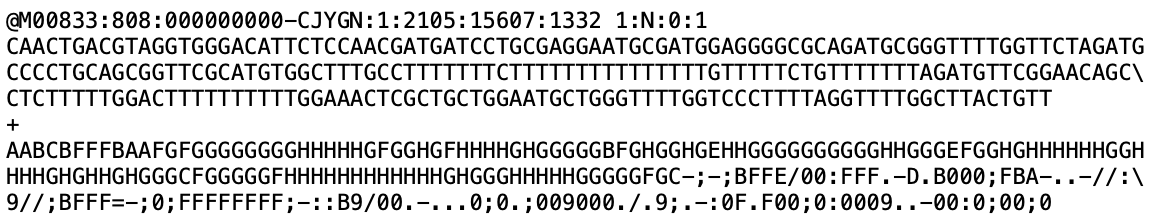
\includegraphics[width=0.8\textwidth]{figures/fastq-example.png}
%  \caption{Example of the four lines in a FASTQ entry.}
%  \label{fig:fastq-example}
%\end{figure}

%\subsection{General Feature Format - GFF}
%General feature format (GFF) is a popular format for storing
%information about features relative to a position on an genetic
%sequence, and comprises a large portion of annotation results from
%this work. These features can be whatever the user desires, as long as
%the feature entry follows the required GFF guidelines. Relative to a
%reference sequence, each GFF entry contains the following
%tab-delimited columns: sequence ID, source, feature type, start
%position, end position, score, strand, phase, and a semi-colon
%delimited list of attributes. GFF files are widely supported accross
%bioinformatics tools, making them highly versatile while also
%remaining relatively simple in nature but also allowing for storage of
%more complicated items via the attributes column. One significatn
%useage of GFF files is in visualization of features against the
%reference sequence from which they were derived. Most genome viewers
%(or browsers) support GFF files as input, allowing intuitive
%visualization of many features when overlayed on a reference
%sequence. An example of a GFF entry can be seen in
%figure~~\ref{fig:gff-example}.

%\begin{figure}
%  \centering
%  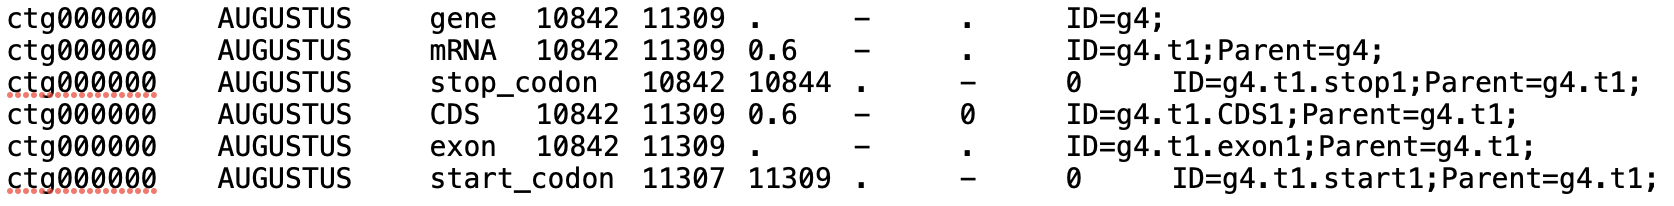
\includegraphics[width=0.8\textwidth]{figures/gff-example.png}
%  \caption{An example of GFF entries for a single gene.}
%  \label{fig:gff-example}
%\end{figure}

%\section{BLAST and tblastn}
%The basic local	alignment search tool (BLAST)~\ref{Altschul1990}	has
%been a popular tool in the bioinformatics space, used to align
%biological sequences and measure their similarity. The original	blast
%program was developed for alignment of nucleotide sequences, but other
%blast tools have been developed as well. One of these tools is tblastn
%which was developed to align reverse-translated protein sequences to
%another nucleotide sequence. To align the protein sequences, the query
%nucleotide sequences are translated in all six reading frames and then
%aligned to the proteins.  Tblastn is particularly useful for
%identifying functional or conserved proteins in	a nucleotide sequence.

%\section{BUSCO}
%The Benchmarking Universal Single-Copy Orthologs
%(BUSCO)~\ref{10.1093/bioinformatics/btv351} tool was developed to
%evaulate assemblies and subsequent annotations from the perspective of
%gene orthology. As genomes diverge evolutionarily, it is expected that
%some genes will be conserved as they are required for basic
%function. The BUSCO (Benchmarking Universal Single-Copy Orthologs)
%tool and datasets were developed to assess completeness of an
%annotation in comparison to evolutionarily conserved genes.
